\chapter{Evaluation} \label{chap:eval}
\begin{chapquote}{Milton \& Rose D. Friedman, \textit{Free to Choose: A Personal Statement}}
Despite the limited scope of that experiment, giving parents greater choice had a major effect on education quality.
\end{chapquote}

\pengcheng{for each experiment, 4 paragraphs: 1. why are we doing the experiment and what is to show; 2. description of the experimental procedure; 3. describe the results; 4. draw a conclusion}

In this chapter, we evaluate the software and hardware implementation of the proposed FPsPIN platform.  We first describe the platform we implemented FPsPIN on.  We then present an analysis of the hardware components proposed in \Cref{chap:hardware} to identify potential bottlenecks in the hardware design and implementation.  Finally, we demonstrate the overall functionality and performance of the system through several demo applications.

\section{Experiment Setup} \label{sec:eval-setup}

The experiments are done on the AMD server with the Ryzen 7 2700 CPU and the \ac{pcie}-attached Xilinx VCU1525\footnote{\url{https://www.xilinx.com/products/boards-and-kits/vcu1525-a.html}} Development Kit; more details can be found in \Cref{sec:fpga-basics}.  We run the \ac{fpga} board at 16 lanes of \ac{pcie} 3.0 clocked at 8 GT/s.  A diagram of the experiment platform is shown in \Cref{fig:experiment-setup}.  Corundum runs at its native frequency of 250 MHz on the Virtex UltraScale+ \ac{fpga}.  However, we could only run the application block (FPsPIN) at 40 MHz due to the PsPIN IP not being designed for \ac{fpga}s: the \ac{pulp} RISC-V cores are designed for an advanced \ac{asic} process node and have long critical paths on \ac{fpga}s.  As a result, we clock the processing cluster at 40 MHz.

\paragraph{Networking} The two 100 Gbps QSFP Ethernet ports on the \ac{fpga} board are attached via one \ac{dac} cable, forming a loop-back between the two interfaces of Corundum.  Since the two interfaces are present on the same Linux host, we have to isolate the two network interfaces into separate \emph{network namespaces} to avoid a direct loop-back in software.  The exact network topology of the system can be seen in \Cref{fig:experiment-setup}.  A script, \texttt{setup-netns.sh}, automates the creation and tear-down of network namespaces and assignment of the interfaces to them.

\paragraph{Toolchain} We use Ubuntu 20.04.4 LTS on the host with a slightly modified Linux 5.15.0-76-generic kernel with the \ac{cma} enabled; this allows the FPsPIN kernel driver to allocate arbitrarily large contiguous \ac{dma} areas, as is required by demo applications shown later in \Cref{sec:demos}.  We use Xilinx Vivado 2020.2 to produce the \ac{fpga} bitstream, the \ac{pulp} RISC-V toolchain\footnote{\url{https://github.com/pulp-platform/pulp-riscv-gnu-toolchain}} to compile the \ac{spin} handlers, and the Ubuntu system GCC for the host-side applications.

\begin{figure}
    \centering
    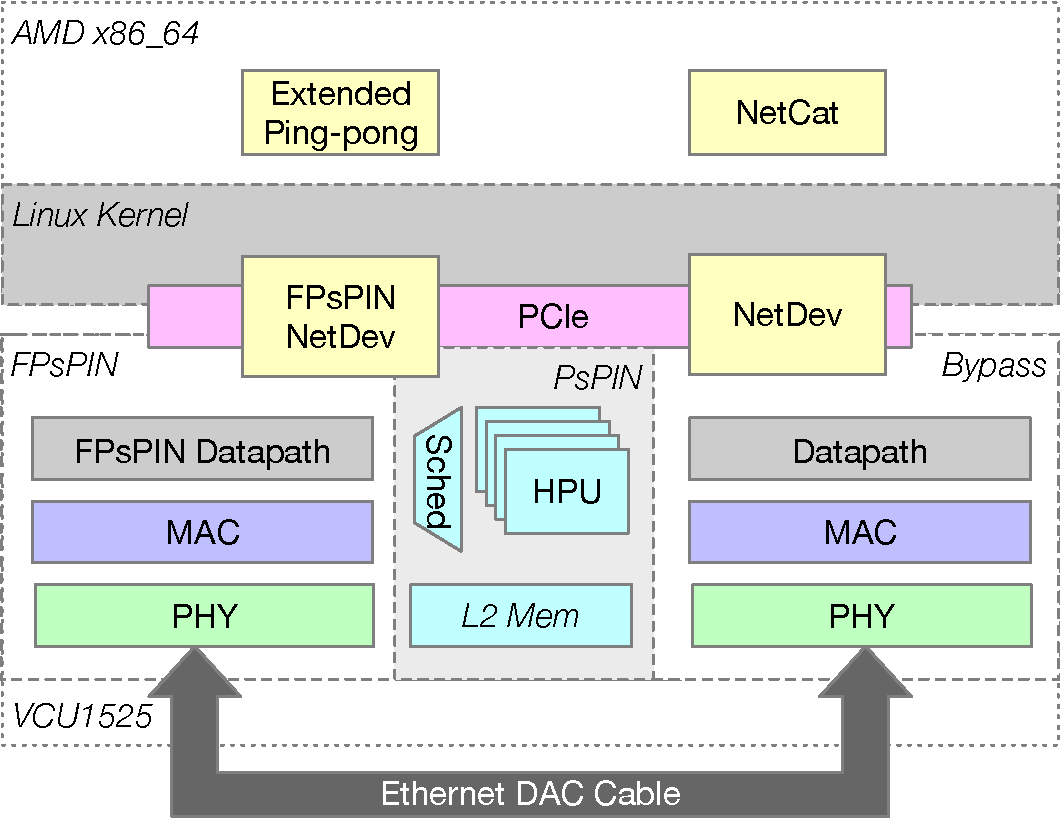
\includegraphics[width=.8\linewidth]{figures/experiment-setup.pdf}
    \caption{The experiment setup.  The \ac{spin} and non-\ac{spin} host applications are in two separate network namespaces to prevent the direct loop-back mechanism in Linux that prevents packets from actually going through FPsPIN.} \label{fig:experiment-setup}
\end{figure}

\section{Design Analysis} \label{sec:hw-analysis}

To evaluate the implementation quality of the newly introduced data-path components, we estimate the theoretical latency of these components as described in \Cref{chap:hardware} based on the \ac{rtl} source.  \Cref{tab:lat-cycles} shows the latency in cycles based on the state machine construction in the Verilog \ac{rtl} code, the frequency, and the latency time in nanoseconds. The \texttt{pspin\_ingress\_dma} module has a latency linearly related to the packet size due to dependency requirements as introduced in \Cref{sec:ingress-datapath}.  We show in the later sections that these latency numbers are negligible compared to other parts of the system and thus would not have a big impact on overall system performance.

\begin{table}[tp]
    \centering
    \begin{tabular}{lccc}
    \toprule
    Module & Cycles & Frequency (MHz) & Latency (ns) \\ \midrule
    Matching engine & 4 & 40 & 100 \\
    Allocator & 0 & 40 & 0 \\
    Ingress \ac{dma} & 8\mytilde{}70 & 40 & 200\mytilde{}1750 \\
    HER generator & 0 & 40 & 0 \\
    Host \ac{dma} & \emph{n/a} & 250 & \mytilde{}450 \\
    \bottomrule
    \end{tabular}
    \caption{Latency estimation for various data path modules in cycles and nanoseconds.  Note that as the host \ac{dma} goes over \ac{pcie} to the host DRAM, the exact latency in cycles is difficult to estimate; the latency in nanoseconds is measured on real hardware via the \ac{ila} on Xilinx platforms.} \label{tab:lat-cycles}
\end{table}

Resource utilisation and timing are very important static insights into \ac{fpga} designs.  While we have trimmed the original PsPIN design significantly compared to the standard configuration~\cite{di_girolamo_pspin_2021} as shown in \Cref{tab:pspin-config}, the design is still very hard to close timing due to congestion issues.  We present in \Cref{tab:design-qor} data in resource utilisation, timing, and time taken to implement the design.  To ensure that we get acceptable implementation results for each run, we employ the \emph{incremental implementation flow}~\cite{noauthor_incremental_nodate} from Xilinx to have the \ac{eda} tool try to reuse routed nets from previous valid implementation runs.  This shortens implementation time and improves the general \ac{qor} of the resulting design.

\begin{table}[tp]
    \centering
    \begin{tabular}{lcc}
    \toprule
    Resource Category & \cite{di_girolamo_pspin_2021} & \textbf{FPsPIN} \\ \midrule
    Clusters & 4 & 2 \\
    \#\ac{mpq} & 256 & 16 \\
    L1 Cluster Memory & 1 MiB & 256 KiB \\
    L2 Program Memory & 32 KiB & 32 KiB \\
    L2 Packet Memory & 4 MiB & 512 KiB \\
    L2 Handler Memory & 4 MiB & 1 MiB \\
    L2 SRAM Latency (cycles) & 1 & 1 \\
    \bottomrule
    \end{tabular}
    \caption{Comparison between the stock PsPIN configuration and that used in FPsPIN.  The \ac{mpq} enables parallel in-flight messages; by reducing the number of queues available, we limit the number of concurrent in-flight messages to 16.} \label{tab:pspin-config}
\end{table}

\begin{table}[tp]
    \centering
    \begin{tabular}{ccc}
    \toprule
    \ac{qor} Metric & \multicolumn{2}{c}{Value} \\ \midrule
    \ac{lut} & 649k & 54.9\% \\
    \ac{ff} & 499k & 21.1\% \\
    \ac{bram} & 1141 & 52.8\% \\
    \ac{uram} & 206 & 21.5\% \\
    \ac{wns} (ns) & \multicolumn{2}{c}{-0.126} \\
    \ac{tns} (ns) & \multicolumn{2}{c}{-37.958} \\
    Impl. Time & \multicolumn{2}{c}{7:01:46} \\
    \bottomrule
    \end{tabular}
    \caption{\ac{qor} metrics of the hardware implementation of FPsPIN.  The first four entries (\ac{lut}, \ac{ff}, \ac{bram}, \ac{uram}; refer to \Cref{sec:fpga-basics}) denote key resource consumption and the percentage utilisation value on the VU9P device; \ac{wns} and \ac{tns} measure how much the design has failed timing.} \label{tab:design-qor}
\end{table}

\section{Demo Applications on Real Hardware} \label{sec:demos}

We present three \ac{e2e} demo applications to showcase the real-world programmability and performance of FPsPIN.  We show that it is possible to write arbitrary packet-processing applications for the platform with the first two applications, \emph{ping-pong} and the \ac{slmp} file transfer.  We further characterise the performance of the platform in detail with the \ac{mpi} Datatypes demo.

\pengcheng{the two pingpong demos are functional demos that exercise different components; slmp file transfer is a synthetic benchmark to measure throughput and show \ac{slmp}-based message boundaries; datatypes show the overlapping, latency, and bandwidth characteristics of a real-world application}

\subsection{Ping-pong}

\paragraph{Motivation} We demonstrate the overall system functionality with two classic types of \emph{ping-pong} protocols: \ac{icmp} and \ac{udp}.  With this demo, we exercise the various data-path and control-path components newly introduced in FPsPIN to show their basic functionality.  In addition, we evaluate the system \ac{e2e} \ac{rtt} under simple packet processing workloads to compare with pure-CPU processing.  We further identify \ac{rtt} contributions from different actors in order to evaluate bottlenecks in the system.

\paragraph{Experiment} We implement on FPsPIN the server to respond to client requests; the operation flow of the server is shown in \Cref{fig:demo-pingpong}.  Both protocols operate in the same way that the client sends a request packet and the server sends back a response.  The server needs to swap the source and destination addresses in the Ethernet, IP, and \ac{udp} headers, and recalculate relevant checksums.  For each protocol, we implement three different modes of operation:
\begin{itemize}
    \item the \emph{baseline} a.k.a.\ host-only case (\textbf{Host}): all processing on the CPU by setting the FPsPIN matching engine to bypass mode;
    \item the \emph{FPsPIN-only} case (\textbf{FPsPIN}): FPsPIN does all the packet processing (header processing and checksum calculation);
    \item the \emph{combined} case (\textbf{Host+FPsPIN}): FPsPIN swaps the addresses in the headers and the host CPU calculates checksums.
\end{itemize}
We use the \texttt{ping} utility from \emph{iputils}~\cite{noauthor_iputilsiputils_2023} for \ac{icmp} and \texttt{dgping} from the \emph{stping} suite~\cite{katherine_stpingdgping_2023} for \ac{udp}.  For \textbf{Host} mode, we use the responder in the Linux kernel for \ac{icmp} and the user-space \texttt{dgpingd} for \ac{udp}.  For both the \textbf{FPsPIN} and \textbf{Host+FPsPIN} modes, we use the same naive IP checksum algorithm implementation.

An important difference between the \ac{udp} and \ac{icmp} ping protocols is that \ac{icmp} requires the \emph{entire payload} to be included in the calculation of the checksum field, while \ac{udp} only specifies an \emph{optional} checksum of the \emph{\ac{udp} header}; we omit this header checksum in our \ac{udp} ping server implementation on FPsPIN.  This difference between the two protocols impacts both the server and client implementation, but is especially significant for the server since the \ac{rtt} measurements taken at the client do not include packet preparation and checksum validation time on the client side.

\begin{figure}
    \centering
    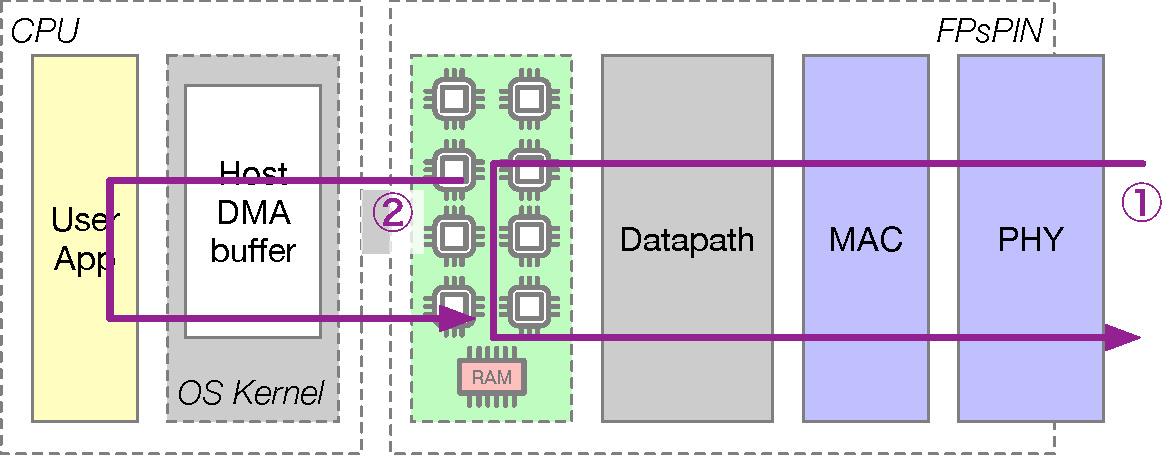
\includegraphics[width=.8\textwidth]{figures/demo-apps.pdf}
    \caption[Workflow of the ping-pong demo]{Workflow of the two ping-pong applications.  \circled{1}) Normal operation; the cluster processes incoming ping requests and sends back responses (\textbf{FPsPIN}).  \circled{2}) The cluster can optionally choose to forward data to the host application for further processing (\textbf{Host+FPsPIN}).} \label{fig:demo-pingpong}
\end{figure}

For both \ac{icmp} and \ac{udp} and the three modes of operation, we measure the \ac{e2e} \ac{rtt} of the ping-pong process from the client by running the ping program 20 times, taking 100 measurements in each iteration.  This would take into consideration any possible interference between the ping client and server that would result in variance in the measurement, as well as to allow caches to warm up.  We plot this \ac{e2e} \ac{rtt} with their medians and 95\% confidence intervals calculated with the bootstrap method~\cite{diciccio_bootstrap_1996} in \Cref{fig:pingpong-lat}.  In addition in cases that involve FPsPIN, we measure cycle counts in the handler code to time the mean handler execution time and latency of host processing.  We plot a breakdown of the \ac{e2e} \ac{rtt} in these cases in \Cref{fig:pingpong-breakdown}.

\begin{figure}[tp]
    \centering
    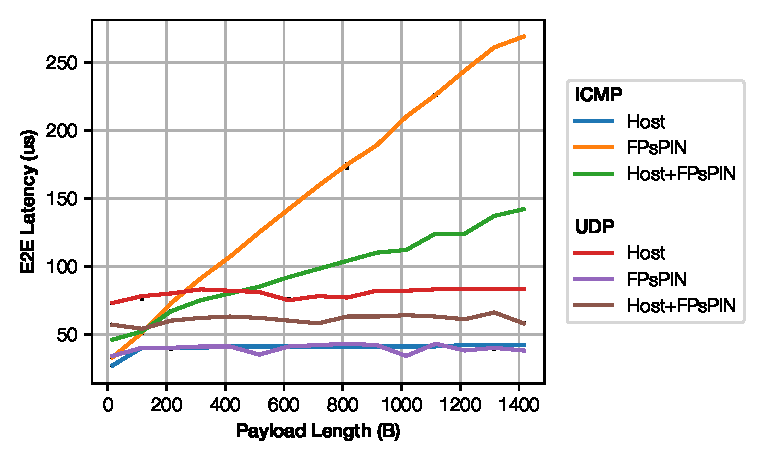
\includegraphics{thesis/figures/pingpong-lat.pdf}
    \caption{Median \ac{e2e} \ac{rtt} of both protocols across the three setups.  The error bars in black show the 95\% confidence interval.} \label{fig:pingpong-lat}
\end{figure}

\begin{figure}[tp]
    \centering
    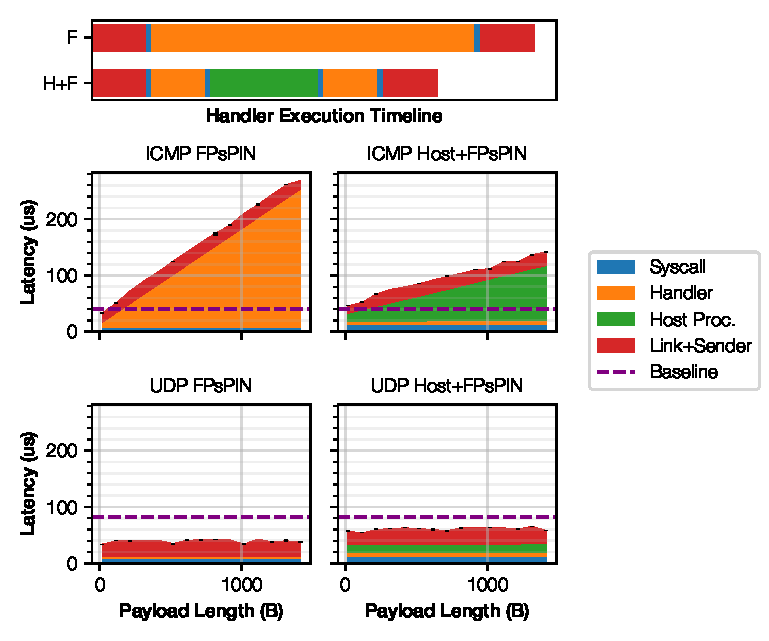
\includegraphics{thesis/figures/pingpong-breakdown.pdf}
    \caption{Breakdown of the \ac{e2e} \ac{rtt} into different categories.  The timeline at the top shows the time-series relationship between the various time components: \emph{Syscall}, time spent reading the cycles counter from trapping into M-mode; \emph{Handler}, time spent executing the packet handlers, excluding waiting for host; \emph{Host Proc.}, time spent waiting for host DMA and processing on the CPU; and \emph{Sender}, time spent on the Ethernet wire and client side.  \emph{Baseline} marks the median \ac{e2e} \ac{rtt} in \textbf{Host} mode.} \label{fig:pingpong-breakdown}
\end{figure}

\paragraph{Data interpretation} A key observation we make is that both \textbf{FPsPIN} and \textbf{Host+FPsPIN} performed significantly better than \textbf{Host} for \ac{udp}.  This is mainly due to the packet data in FPsPIN modes not having to get \ac{dma}'ed to host memory, context switch to user-mode on the CPU, and go through the Linux \ac{udp} network stack.  The overhead of the context switch and the \ac{udp} stack can be confirmed with a comparison between \ac{udp} and \ac{icmp} in \textbf{Host} mode, showing a difference of \mytilde{}41 us.  As we see in \Cref{fig:pingpong-breakdown} in \textbf{Host+FPsPIN} for \ac{udp}, our system reliably achieves a \mytilde{}20 us \ac{rtt} advantage over the baseline case even with the added latency from host processing.  In addition, we notice that in all four cases with FPsPIN the \emph{syscall} category occupies 10\mytilde{}20 us in the \ac{rtt}.  As we have previously explained in \Cref{sec:handler-runtime}, this added latency is due to a lack of user-mode accessible cycle counters and should be easily fixed in future work.

We notice a big divergence in the course of \ac{e2e} \ac{rtt} w.r.t.\ payload size between \ac{icmp} and \ac{udp} in \Cref{fig:pingpong-lat}: in the two modes that involve FPsPIN for \ac{icmp}, the \ac{rtt} increases almost linearly with the payload size; while in the \textbf{Host} mode for \ac{icmp} as well as all three modes for \ac{udp},  the \ac{rtt} remains relatively constant.  This reflects the difference in checksum calculation between the \ac{icmp} and \ac{udp} ping protocols, showing that checksum calculation time is a significant component of the \ac{icmp} response \ac{rtt}.  A comparison between the \textbf{Host+FPsPIN} and \textbf{Host} modes for ICMP in \Cref{fig:pingpong-breakdown} reveals that the Linux kernel's \ac{icmp} responder uses extremely optimised code paths, highlighting room of improvement in our IP checksum algorithm.

We further observe that the lower frequency that \ac{pulp} cores in FPsPIN run at have a significant impact on packet processing latency.  This is confirmed by \Cref{fig:pingpong-breakdown} between \emph{Handler} on \text{FPsPIN} and \emph{Host Proc.} on \text{Host+FPsPIN} for \ac{icmp}.  It shows that a single core on FPsPIN is \emph{only} \mytilde{}2.8x slower than a single CPU core, a gap way smaller than the actual performance difference between these cores (40 MHz vs 3.4 GHz).  Part of this small performance gap comes from the fact that the host CPU performance in checksum calculation is far from ideal due to the CPU always issuing uncached requests to the host DRAM as a result of a lack of cache-coherency over \ac{pcie}.  In addition, the host processing category also includes one \ac{pcie} \ac{rtt} between the host CPU and FPsPIN and polling latency, both of which are not present on FPsPIN.

\paragraph{Conclusion} The \ac{rtt} advantage from FPsPIN against the CPU-only \textbf{Host} case shows that FPsPIN allows packet processing with lower latency, thanks to its proximity to the data and lack of context switch overheads.  The \ac{icmp} cases show that FPsPIN still has plenty of potential for higher performance in packet processing from a faster core built for \ac{fpga}s, optimised code that reduces handler execution time, and domain-specific accelerators for compute-heavy workloads like checksum calculation.

\subsection{\acs{mpi} datatypes} \label{sec:mpi-datatypes-demo}

\paragraph{Motivation} Apart from synthetic benchmarks like the ping-pong demo we showed in the previous section, we also need to demonstrate the ability of FPsPIN to run real-world \ac{spin} workloads.  \Ac{mpi} Datatypes~\cite{pierce_types_2002} is a popular mechanism for exchanging custom messages over the \ac{mpi} paradigm commonly used in parallel computing.  On the sender side, the datatypes subsystem in \ac{mpi} \emph{serialises} the custom message with non-contiguous memory blocks (in other words, \emph{holes} in between) into a contiguous \emph{streaming} buffer for transmission on the network; on the receiver side, \ac{mpi} \emph{deserialises} the contiguous message back into the non-contiguous messages for the user application.

Previous work on \ac{spin} has ported the \emph{MPICH dataloop}-based single-threaded implementation of MPI Datatypes to \ac{spin} handlers that run on a simulator-based platform~\cite{di_girolamo_network-accelerated_2019}.  By porting these existing \ac{spin} handlers to FPsPIN, we characterise the throughput of \ac{spin} workloads on FPsPIN with different levels of handler complexity on the platform.  In addition, we showcase the ability of FPsPIN to achieve almost perfect \emph{computation/communication overlap} with a compute-heavy CPU workload that runs simultaneously.  Last but not least, since MPI Datatypes requires to send messages of arbitrary length on the network, we demonstrate the operation of the SLMP protocol introduced in \Cref{sec:slmp}.

\paragraph{Experiment} We port the handlers in~\cite{di_girolamo_network-accelerated_2019} to the FPsPIN platform.
A major difference between the original target platform and FPsPIN is the underlying network layer: the handlers were designed for InfiniBand-style networks that offer a \emph{reliable message transport} with arbitrary length support, while FPsPIN runs on top of lossy Ethernet; we have analysed this difference in network-layer guarantees in detail in \Cref{sec:slmp}.  For MPI Datatypes, we encapsulate the serialised buffer in \ac{slmp} messages on the sender side and send back \ac{ack} packets in the handler.  In addition to the \ac{slmp} encapsulation, we modify the original handlers to call correct host DMA and host notification functions offered by the FPsPIN runtime. 

Due to the single-threaded nature of the \emph{dataloop} implementation of MPI Datatypes, we are unable to implement \emph{packet-level parallelism} and are thus forced to use a sender window size of 1 packet to ensure serialised packet processing; this has severe performance implications as we discussed in \Cref{sec:slmp}.  To make use of all the 16 \ac{hpu}s on FPsPIN, we implement \emph{message-level parallelism}, sending multiple messages in parallel.  The handler function stores all per-message states in the shared L2 handler memory and selects the correct per-message state according to the \ac{slmp} message ID.  We evaluate the \ac{e2e} bandwidth of datatype handlers on FPsPIN in comparison to the reference MPICH datatypes implementation on CPU with varying degrees of parallelism in \Cref{fig:datatypes-tput}.

\begin{figure}[tp]
    \centering
    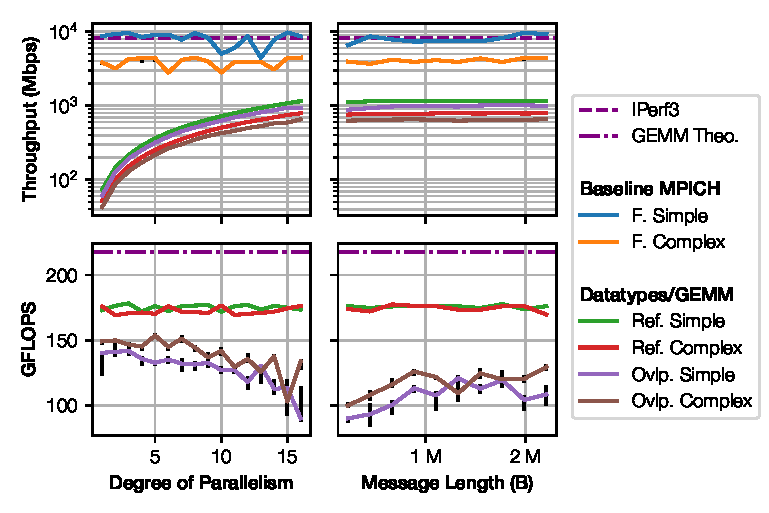
\includegraphics{thesis/figures/datatypes-tput.pdf}
    \caption{Comparison of median datatypes \ac{e2e} throughput between the MPICH reference CPU implementation (baseline) and on FPsPIN.  We run the baseline on both vanilla Corundum i.e.\ without PsPIN as well as FPsPIN to show any potential slow-downs to normal NIC operation from introducing PsPIN.  The error bars in black show the 95\% confidence interval.} \label{fig:datatypes-tput}
\end{figure}

To demonstrate the \emph{computation/communication overlap} capability of FPsPIN, we run double-precision \ac{gemm} from OpenBLAS~\cite{xianyi_model-driven_2012} on the CPU to simulate a compute-heavy workload that runs simultaneously with the datatypes deserialisation on FPsPIN.  Since the CPU fetches notifications from FPsPIN in poll mode (\Cref{sec:sw-lib}), it is the best to poll as few times as possible to avoid wasting CPU cycles that could otherwise be running the computation workload.  The regularity of \ac{hpc} workloads, which allows \emph{estimating} the time a communication task takes to finish.  For a meaningful evaluation of computation/communication overlap, we \emph{tune} the \ac{gemm} size for a \emph{balanced} setup between computation and communication, i.e.\ to minimise both datatypes latency and polling overhead.  We show in \Cref{fig:datatypes-tuning-goal} the two opposites of polling frequency, both of which hurts the performance of either the datatypes or \ac{gemm}.  By tuning the size of a single invocation of \ac{gemm}, we find the sweet spot to balance between these two situations.  We report the \emph{overlap ratio} in \Cref{fig:datatypes-overlap}, defined as the following:

\[
\text{OverlapRatio} = \frac{T_{\text{GEMM}}}{T_{\text{GEMM}} + T_{\text{Poll}}}
\]

\begin{figure}[tp]
    \centering
    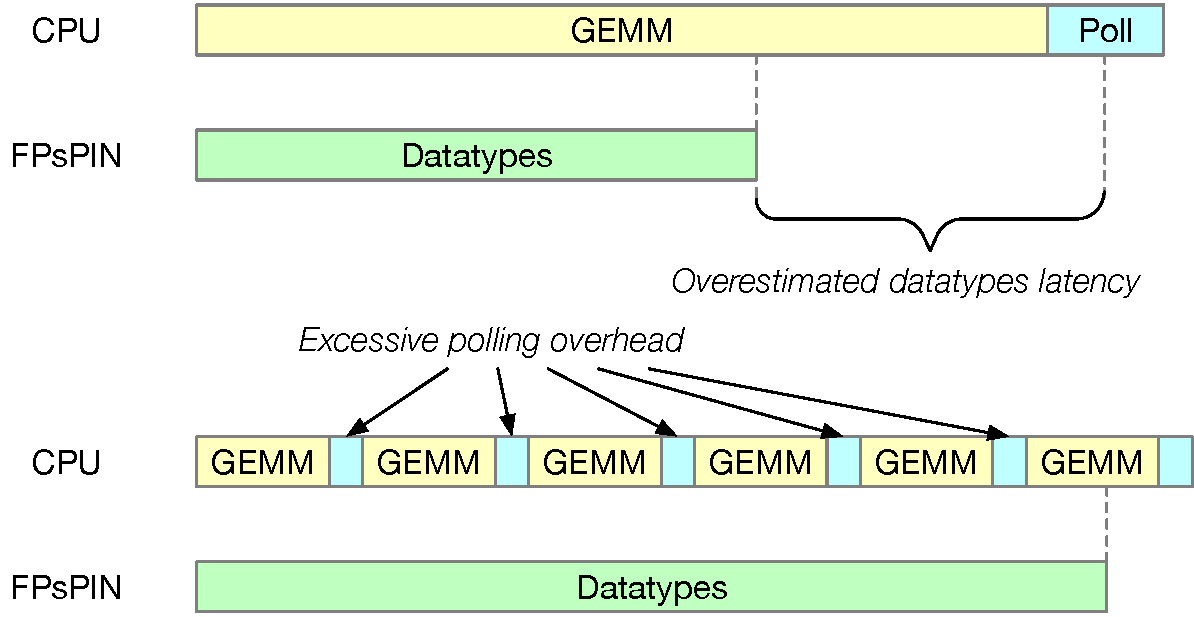
\includegraphics[width=.8\textwidth]{thesis/figures/datatypes-tune-goal.pdf}
    \caption{Two possible situations of overlap between \ac{gemm} and datatypes processing.  The top case imposes excessive latency on datatypes processing due to not polling at a high-enough frequency; the bottom case imposes excessive overhead on the \ac{gemm} workload due to polling too frequently.} \label{fig:datatypes-tuning-goal}
\end{figure}

\begin{figure}[tp]
    \centering
    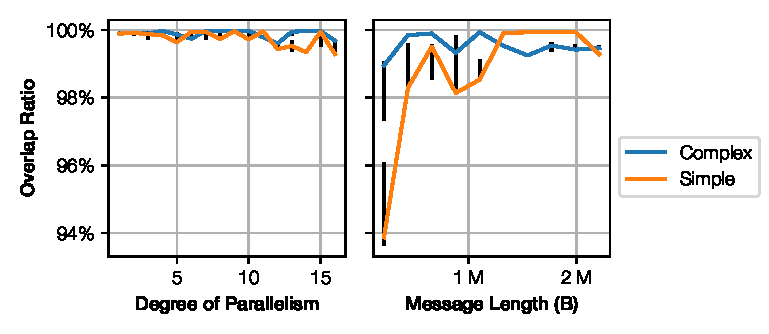
\includegraphics{thesis/figures/datatypes-overlap.pdf}
    \caption{} \label{fig:datatypes-overlap}
\end{figure}

In order to have correlated timing measurements between datatypes processing and \ac{gemm}, we measure the time elapsed for both workloads on the receiver side.  Since the host application does not get a notification until the datatypes transfer is finished, we introduce a \ac{rts} signal from the receiver to the sender: the receiver application sends \ac{rts} to the sender and starts the \ac{gemm} workload on CPU.  We take the time between the notification from FPsPIN and the \ac{rts} as the elapsed time for the datatypes workload.

\paragraph{Data interpretation}

\paragraph{Conclusion}

\pengcheng{message-level parallelism; 1. make handlers stateless; a) we replay segments on every packet b) ideally we get rid of the MPICH segments data structure with the compiled datatypes paper impl.  2. allocate dynamically the per-message state (to support arbitrary number of messages).  3. have a fixed number of message states for all in-flight messages and spill to the host if we have too many (picked)}

\pengcheng{possible performance optimisations/current limitations: bank conflicts accessing datatypes dataloop state in L2; lower bandwidth by \ac{dma}-ing from L1 instead of L2.  (do we actually talk about these?)}

\subsection{\acs{slmp} file transfer}

\paragraph{Motivation} As we have seen in the MPI datatypes benchmark in \Cref{sec:mpi-datatypes-demo}, the throughput of packet processing depends highly on the complexity of the packet handlers.  It is thus difficult to evaluate the real throughput capacity of FPsPIN with the datatypes handlers due to its various implementation limits.  In this demo application, we show the throughput of FPsPIN through a simple file transfer: the sender transmits a file encapsulated in \ac{slmp} and the receiver posts the segments to the host CPU for storing.  With no requirement of serialised access to per-message states, we evaluate the full potential of \emph{packet-level parallelism} of FPsPIN.

The MPI datatypes demo forced a flow control window size of 1 packet due to the serialisation requirements.  However, \ac{slmp} as discussed in \Cref{sec:slmp} offers flexible window size and sender parallelism configurations.  We evaluate the performance trade-offs of different sender configurations and identify the best configuration for other applications.  In addition, we explore the consequences on packet processing from unreasonable flow control configurations.

\paragraph{Experiment} We implement packet handlers that, upon receiving a \ac{slmp} segment, \ac{dma} the segments to the correct offset in the host memory according to the \ac{slmp} message offset field in the packet header.  After processing the last packet with the \ac{eom} bit, the tail handler posts a notification to the host application, which then saves the host \ac{dma} buffer into a file.  The sender transmits the file with the \ac{slmp} and records the elapsed time for throughput calculation.  We report the throughput progressions with diverse file sizes and sender configurations in \Cref{fig:slmp-tput}.

\begin{figure}[tp]
    \centering
    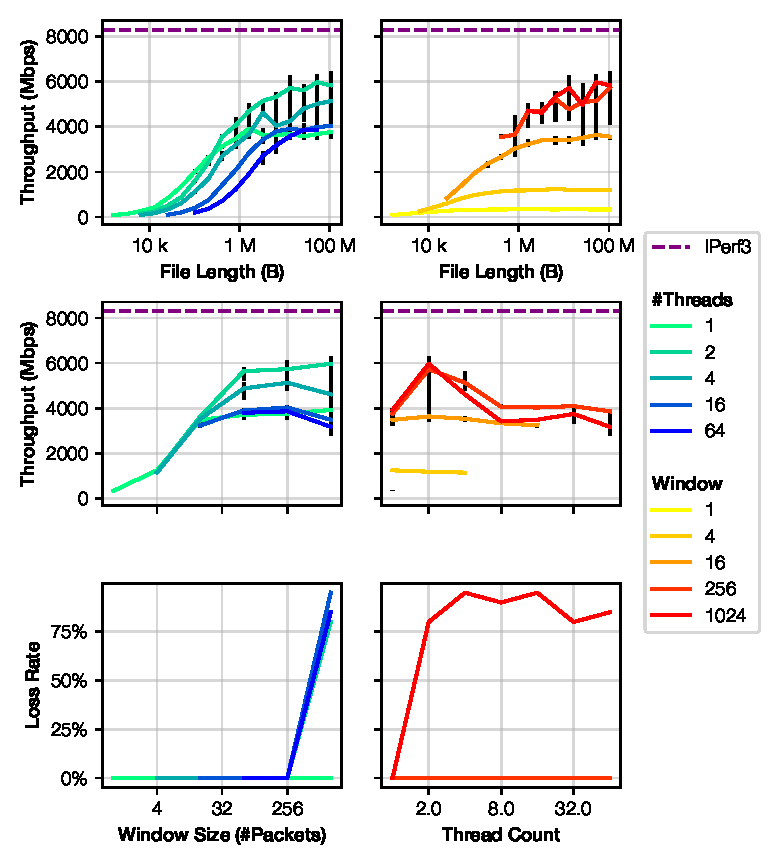
\includegraphics{thesis/figures/slmp-tput.pdf}
    \caption{Median throughput of both protocols across different sender-side window size and parallelism configurations.  The top left plot shows the best throughput across different window sizes; the top right across different thread counts; the bottom two across different file lengths.  Each data point comes from 20 successful \ac{slmp} message deliveries; the error bars in black show the 95\% confidence interval.} \label{fig:slmp-tput}
\end{figure}

As we discussed in \Cref{sec:slmp}, a flow control window too big will result in packet loss at the receiver and thus a failure in message delivery.  To explore how the flow control settings affect message delivery, we plot the failure rate of message delivery at different sender settings in \Cref{fig:slmp-loss}.  For each configuration, we run the sender for at most 200 times in an attempt to gain 20 successful runs in total.

\begin{figure}[tp]
    \centering
    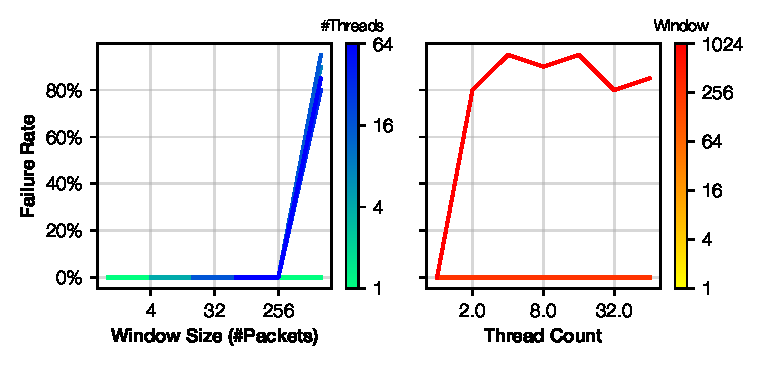
\includegraphics{thesis/figures/slmp-loss.pdf}
    \caption{Failure rate of \ac{slmp} transmissions under different window size and sender thread count configurations.} \label{fig:slmp-loss}
\end{figure}

\paragraph{Data interpretation}

\pengcheng{window size should go only till 256, the number of 1536-byte slots in the packet allocator}
\pengcheng{window size close to 256: loss at large messages? possible cause: lag between \ac{ack} sent and actual reclaim of packet buffer}

\paragraph{Conclusion}

\pengcheng{parallel file receival - e2e bandwidth measurement}
\pengcheng{different operating modes (w/ and w/o \ac{ack} per msg or per packet) of \ac{slmp}}
